\documentclass[11pt]{article}
    \title{\textbf{Práctica 2}}
    \author{Eduardo Salazar del Rio}
    \date{}
    
    \addtolength{\topmargin}{-3cm}
    \addtolength{\textheight}{3cm}
    \usepackage{graphicx}
\begin{document}

\maketitle
\thispagestyle{empty}

\section{Autómata Finito Determinista}
Un autómata finito determinista (AFD) es una 5-tupla (K, Σ, δ, s, F),donde:
K es un conjunto no vacío de estados {q0, q1, q2} \\
\sum $ es un alfabeto$ \{a, b\}\\
$s \in K$ es el estado inicial q0\\
$F  \subseteq K$ es el conjunto de estados finales {q1}\\
$\delta : K x \sum \longrightarrow K$ es la función de transición\\
$\delta : (q0, a, q1), (q0, b, q2), (q1, a, q2), (q1, b, q2), (q2, a, q2), (q2, b, q2)$$

\subsection{Ejemplo Autómata en JFLAP} 

    \begin{example}
    \centering
    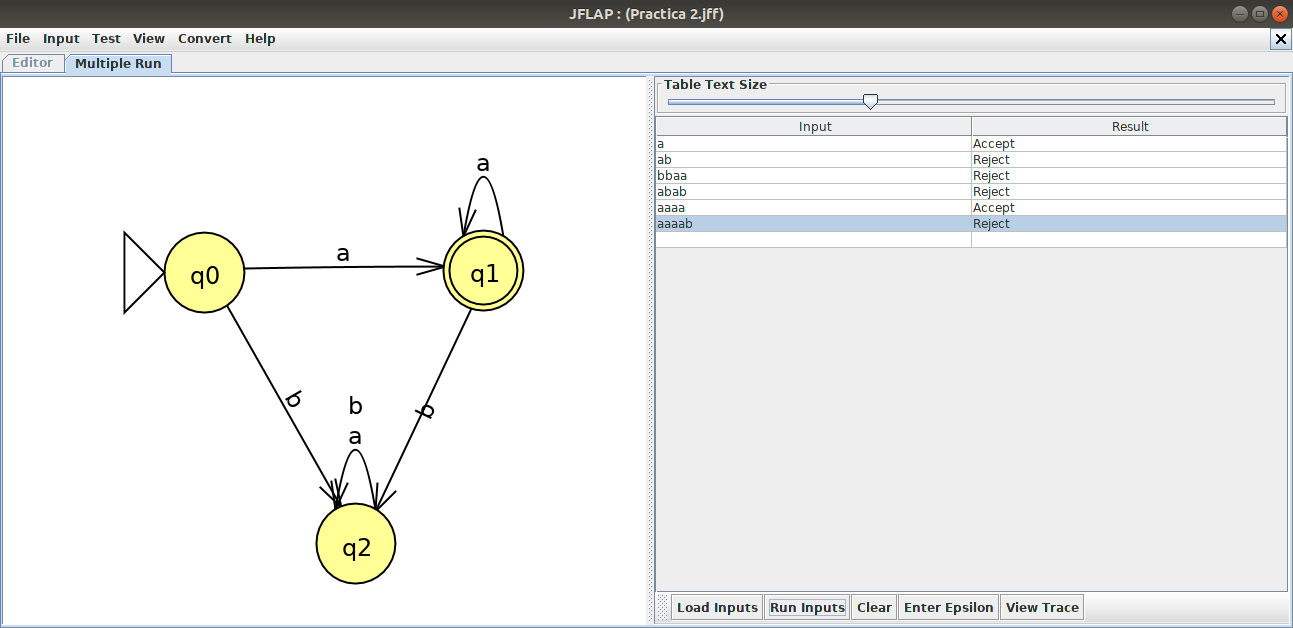
\includegraphics[width=0.80\textwidth]{Automata.jpg}
    \\
    \label{fig:my_label}
    \end{example}

\\
\RaggedRight
\subsection{Ejemplo en Oracle}

    \begin{example}
    \centering
    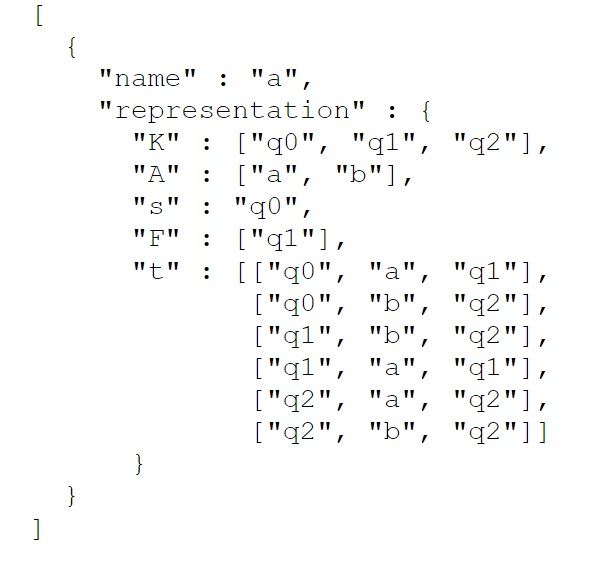
\includegraphics[width=1.0\textwidth]{Prac2.jpg}
    \\
    \label{fig:my_label}
    \end{example}


\end{document}